%%%%%%%%%%%%%%%%%%%%%%%%%%%%%%%%%%%%%%%%%%%%%%%%%%%%%%%%%%%%%%%%%%%%%%%%%%%%%%%
%optimization.tex: Detector Optimization
%%%%%%%%%%%%%%%%%%%%%%%%%%%%%%%%%%%%%%%%%%%%%%%%%%%%%%%%%%%%%%%%%%%%%%%%%%%%%%%%
\chapter{Detector Design and Optimization}
\label{optimization_chapter}
%%%%%%%%%%%%%%%%%%%%%%%%%%%%%%%%%%%%%%%%%%%%%%%%%%%%%%%%%%%%%%%%%%%%%%%%%%%%%%%%

\ac{EBEX} employed a kilopixel array of \ac{TES} bolometers. 
These types of detectors are used on ground-based experiments, like XXX, XXX, and XXX. 
We modified the design in order to optimize the detectors to take advantage of the space-like environment in which \ac{EBEX} was flown.

%%%%%%%%%%%%%%%%%%%%%%%%%%%%%%%%%%%%%%%%%%%%%%%%%%%%%%%%%%%%%%%%%%%%%%%%%%%%%%%%
% TES Bolometer Theory {{{
%%%%%%%%%%%%%%%%%%%%%%%%%%%%%%%%%%%%%%%%%%%%%%%%%%%%%%%%%%%%%%%%%%%%%%%%%%%%%%%%
\section{Bolometer Theory}
\label{sec:tes_bolometer}
%%%%%%%%%%%%%%%%%%%%%%%%%%%%%%%%%%%%%%%%%%%%%%%%%%%%%%%%%%%%%%%%%%%%%%%%%%%%%%%%

%\textcolor{red}{Acronyms is failing us ... the figure descriptions are the first place they appear ... how do we fix this??? FIXED... BUT DON'T REMEMBER HOW :/}

\textcolor{red}{Describe how a bolometer works. Power to temperature detector.}
% Need: cartoon. }

A bolometer is an absorber with some heat capacity weakly coupled to a bath. 
Bolometers measure temperature changes due to power absorption. 
The heat capacitive element absorbs radiation, warms up, and the change in temperature is measured with a thermistor.  
A \ac{TES} bolometer has a superconducting metal as its thermistor. 
The \ac{TES} is called such because it is operated on the edge of its superconducting transition, where there is a steep change in resistance as a function of temperature. 


\textcolor{red}{Figure out how to properly add Mather 1982 applied optics bolometer noise paper to bibfile and reference.}

\begin{figure}[ht!]
\begin{center}
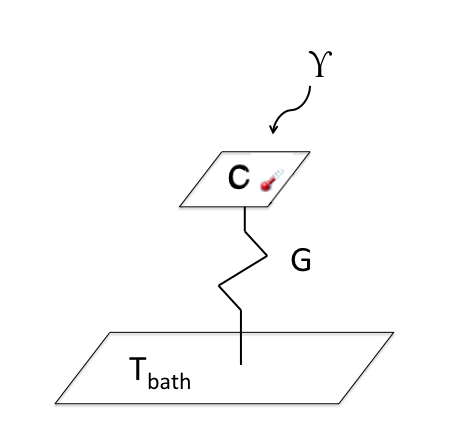
\includegraphics[height=2.5in]{figures/bolometer_cartoon}
\caption{Bolometer. 
\label{fig:bolometer_cartoon} }
\end{center}
\end{figure}


Describe TES.  
\begin{figure}[ht!]
\begin{center}
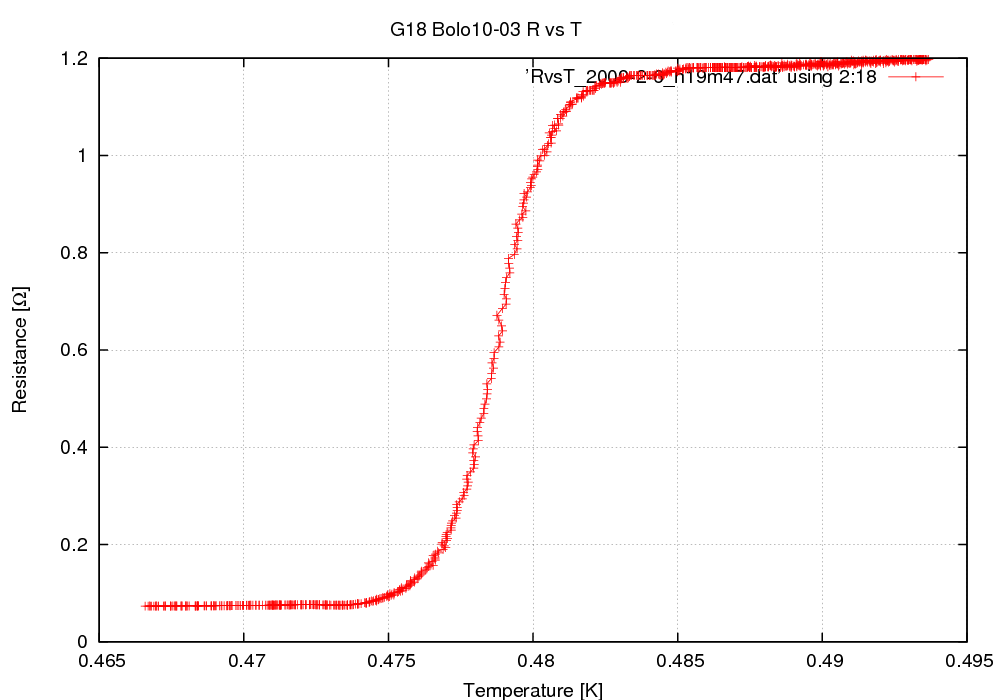
\includegraphics[height=2.5in]{figures/G18_bolo10-03_RvsT_oral}
\caption{Resistance versus temperature for an \ac{EBEX} bolometer.
\label{fig:r_vs_t} }
\end{center}
\end{figure}



\textcolor{red}{Four noise sources, fundamental limit set by photon arrival stats}

1. Electronic/Readout

2. Johnson

3. Phonon (ballistic vs �?)

4. Photon (a. Poisson process, b. Shot noise)



The sensitivity of the instrument is quantified by the \ac{NEP}. 
\ac{NEP} is defined as the absorbed power required to produce a signal-to-noise ratio of one in an electrical bandwidth of one~Hz. 
%not important?
%Note, sometimes \ac{NEP} is instead defined as the \textit{incident} power required to produce a signal-to-noise ratio of one in an electrical bandwidth of one~Hz, \textcolor{red}{cite who??}.
The predicted detector \ac{NEP}, $N$, is given by 
\begin{equation}
N^{2} = N_{photon}^2 + N_{phonon}^2 + \frac{1}{S_I^2} ( N_{Johnson}^2 + N_{readout}^2 )
\end{equation}
\begin{equation}
= 2h\nu P_{rad} + \xi \frac{P_{rad}^2}{\Delta \nu} + \gamma 4k_{B} T^2 G + \frac{1}{S_I^2} (\frac{4k_BT}{R} + N_{readout}^2 )
\label{eq:nep}
\end{equation}
where $h$ is Planck's constant, $\nu$ is the center of the observation frequency band, $P_{rad}$ is the radiative power absorbed by the bolometer, $\xi$ is a unitless number between zero and one quantifying the contribution of photon correlation noise, $\Delta \nu$ is the width of the observation frequency band, $\gamma$ is a unitless number between zero and one accounting for the temperature gradient along the link from the \ac{TES} to the bath, $k_{B}$ is Boltzmann's constant, $T$ is the \ac{TES} temperature, $G$ is the bolometer dynamic thermal conductance, $S_{I}$ is the bolometer current responsivity, and $R$ is the \ac{TES} resistance~\citep{Mather1982a}. 



%%%%%%%%%%%%%%%%%%%%%%%%%%%%%%%%%%%%%%%%%%%%%%%%%%%%%%%%%%%%%%%%%%%%%%%%%%%%%}}}



%%%%%%%%%%%%%%%%%%%%%%%%%%%%%%%%%%%%%%%%%%%%%%%%%%%%%%%%%%%%%%%%%%%%%%%%%%%%%%%%
% Detector Design Modifications for Space-Like Environment {{{
%%%%%%%%%%%%%%%%%%%%%%%%%%%%%%%%%%%%%%%%%%%%%%%%%%%%%%%%%%%%%%%%%%%%%%%%%%%%%%%%
\section{Detector Design}
\label{sec:detector_design}
%%%%%%%%%%%%%%%%%%%%%%%%%%%%%%%%%%%%%%%%%%%%%%%%%%%%%%%%%%%%%%%%%%%%%%%%%%%%%%%%

Discuss target detector parameters. Be very clear about which changes were made to fabrication process in order to optimize the detector sensitivity for a space-like environment and for EBEX.

1. Ideal normal resistance.  
The target normal resistance for all bands was 1.5~$\Omega$ in order to ensure the detector, when biased in the transition, remained in the stable regime where the detector electrical bandwidth, determined in part by the resistance, exceeded the \ac{TES} thermal bandwidth by at least XXX (CITE PAPER). 
%THIS HAS NOTHING TO DO WITH A SPACE-LIKE ENVIRONMENT, but it does have to do with optimization of multiplexing! and so it's relevant. 

2. Ideal transition temperature for our bath temperature. 

\textcolor{red}{Need to generate: plot of phonon noise as a function of critical temperature, given a fixed ebex bath temperature of 260~mK.}


The \ac{TES} was a bilayer of titanium atop aluminum. 
The titanium thickness was fixed at $\sim$110~nm. 
Depending on the wafer, the aluminum thickness varied from $\sim$30 to 50~nm. 
The critical temperature was controlled by the aluminum layer thickness, where the thinner aluminum layer provided a lower critical temperature (and also a higher normal resistance). 

The \ac{EBEX} target critical temperature for all observation frequency bands was 440~mK.

3. Ideal thermal conductance and heat capacity of TES/web 

\textcolor{red}{It's not obvious that/why a decrease in radiative load can equate to an increase in detector sensitivity. This needs to be spelled out clearly somewhere. Here?}

Ground-based telescopes must design their detectors to accommodate the radiative load and fluctuations from the atmosphere. 
The average long-duration balloon floats at an altitude of $\sim$120,000~ft, above $\sim$98\% of the atmosphere. 
\textcolor{red}{Fact check that.}
The predicted load for \ac{EBEX} at float was XXX for the 150~GHz observation band. 
%not mentioning 410 here because it's not accessible from the ground and one number is sufficient for comparison purporses
This is a factor of roughly XXX less than the load observed by a ground-based telescope. 
The \ac{EBEX} detectors inherited their initial design from the ground-based telescopes, the South Pole Telescope and the Atacama Pathfinder Experiment. 
In order to take advantage of the decrease in radiative load at float and increase the detector sensitivity, the fabrication goal was to lower the average thermal conductance from the bolometer to the bath by a factor of XXX to XXX~$pW/K$. 
The design goal provided a safety factor of 2.5 in case of unanticipated radiative load or fluctuations.

In order to work towards (achieve?) this goal for the 150~GHz detectors, the spiderweb legs were roughly doubled in length, from 0.5~mm to 1.05~mm, and a couple of them were decreased in width from 17~$\mu m$ to 6~$\mu m$. 
\textcolor{red}{please point to a photograph which shows the spiderweb legs. also, learn how/if it's ok to use other people's photos and credit them.} 



4. Ideal time constant


The \ac{TES} itself is an AlTi bilayer in the shape of a 19 x 19~$\mu m^{2}$ square, Figure~\ref{fig:bling_and_tes}.

\begin{figure}[ht!]
\begin{center}
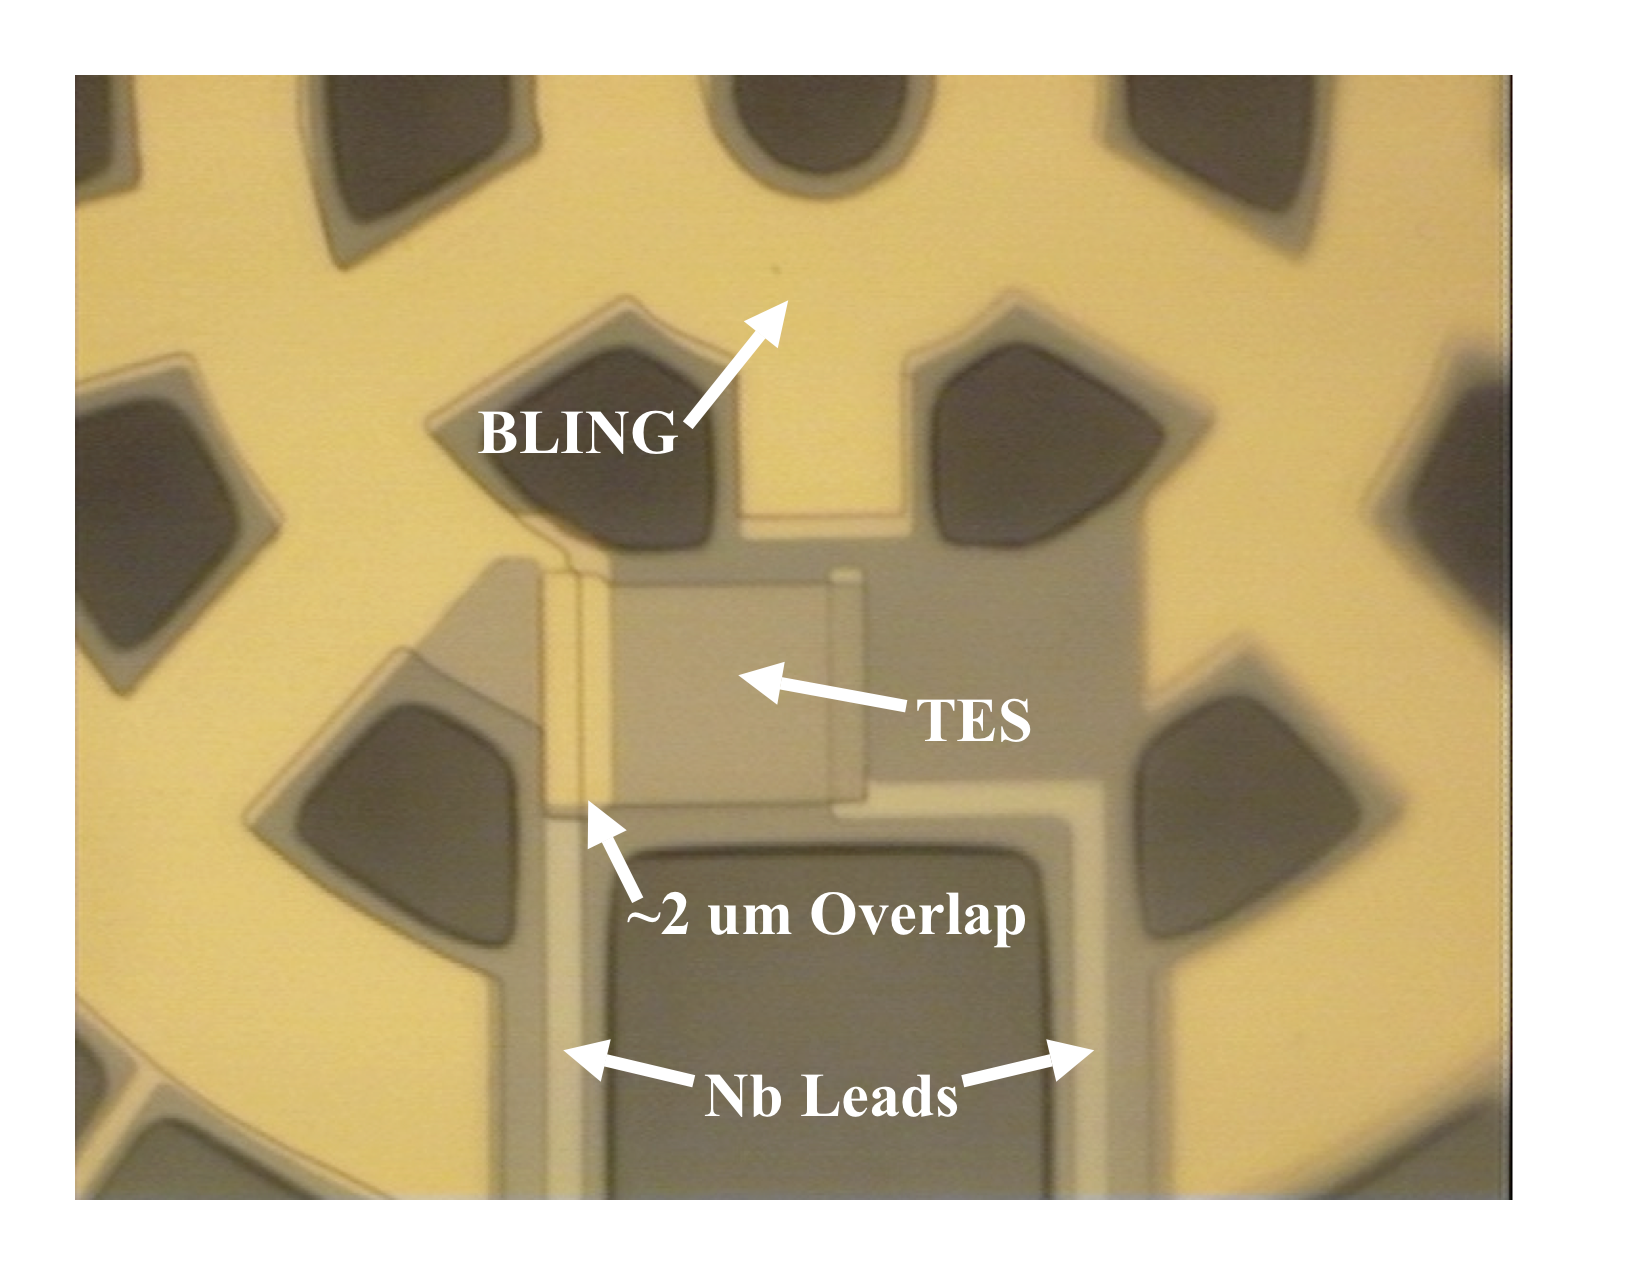
\includegraphics[height=2.5in]{figures/EBEX_BLINGTES_Annotated.png}
\caption{\ac{EBEX} bling and \ac{TES}. Figure courtesy of Benjamin Westbrook. \textcolor{red}{How do I say this is Ben's not mine??}
\label{fig:bling_and_tes} }
\end{center}
\end{figure}

\emph{FROM EMAIL EXCHANGES WITH BEN.
We wanted to decrease G, so we roughly doubled the leg length (where you could find space). Do you have pictures of the mask with the original leg length and the final leg length?
For 150, we pulled out all of the stops we could.  We doubled the length of 7/8 legs from 0.5mm to 1.05 mm. For the 8th leg, we increased it's length by a factor of 3 to 1.45 mm. In addition, we made all the legs expect the one with Nb 6 um wide.  The old design had 2 / 8 with 17 um wide legs. 
We wanted to decrease Tc, so you messed around with the thickness of the Al layer in our Al/Ti TES sandwich. 
Specifically we modulate the thickness of the Al (30-50 nm) compared to the Ti layer, which we held at constant thickness (~110nm). More Al means higher Tc and lower Rn (and converse is true).  Technically it's not a sandwhich (that's Shaul's term) it's just a bilayer, Al with Ti on top. Not Al-Ti-Al nor Ti-Al-Ti.
We wanted to keep the time constant (C/G) the same, so we decreased the heat capacitance by decreasing the thickness of the bling (or we did something else??). 
So we still had a BLING layer (the waffle pattern at the center of the photos).  However, we didn't add any EXTRA gold here like SPT and APEX had.  The C of the EBEX detectors comes from 20 nm of Gold on a 1um thick layer of Silicon nitride.  Where as the SPT/APEX had the 20nm of gold for the web, the 1 um of Silicon Nitrides, + ~500-700 nm of extra BLING only gold at the center.  Since gold has a large heat capacity, it dominates the total C in the detectors.  I attached a quick memo on this I wrote for Shaul that summarized the changes in heat capacity. 
Why did we move away from the circle bling design? 
This is because the waffle pattern has a lower G than the circle so that heat absorbed by the web more efficiently couples to the TES, which ultimately increases optical efficiency (and thus sensitivity) as the TES has time to sense it (i.e it thermalizes) before the heat is dissipated to the bath via the legs.
Does the CPA track speed control the thickness of the Al in the Al/Ti bilayer?
Functionally yes.  There are three knobs one could turn: track speed, target power, and argon pressure.  We chose to modulate thickness by varying the track speed while  trying to keep power and pressure constant.
In the old design, what was the thickness of the other 6 legs?
The old design had 6, 6 micron wide legs and 2, 17 micron wide legs (one with leads and the one opposite the one with leads). 
The one with leads also carried the gold heat link.
> Do you happen to have a schematic that illustrates how we etch the silicon from beneath the silicon nitride? 
This is my talk from the collab meeting eons ago at McGill.  Pages 7-13 describe the fab process in a cartoon sort of way.  It's the closest thing I have to showing how we release the bolometer structures in presentation form.  If you want the full PPT version let me know.  What basically happens is you etch holes/trenches in the silicon nitride layer and then let the wafer sit in a chamber with XeF2 (Xenon DiFlouride), which etches silicon much much faster than it etches silicon nitride.  The gas finds it's way into the holes and starts digging/etching out the silicon.  After some time a pocket is formed underneath the Silicon nitride (I can make a slide showing this if you need) and the XeF2 starts to isotropically etch (not just down by side to side as well) all of the silicon underneath the structure.  Let me know if you need any more help describing this process. 
> Did we have the same goal for Tc for each of our wafers?
> I said it was 1.7 * bath temperature and I think we assumed the bath would be at 270 mK. (giving us a goal of 460 mK)
> Does this magic number 1.7 change with frequency band?
Tc = 1.7* Tbath comes from theory for using dieletrics as a thermal bridge.  The plot attached shows that when n = 3, the optimal Tc (the minimum of the dotted lines) is 1.7 * Tbath. However, we used this is a soft criteria and tune our Tc for psat before we did thermal carrier noise.    That means that we basically did have the same target Tc for each wafer, but that was more to tune Psat rather than noise performance.  We did a pretty good job and found that if Tc was around 480-520  we got the Psats we wanted for our 150 and 250/410 GHz wafers (6-8 and 10-12+ pW) for our mask sets. }




\begin{table}[ht!]
\centering
%\footnotesize
\begin{tabular}{| c | c c | c c | c c |}\hline
\multicolumn{1}{|c}{Band (GHz)}   &  \multicolumn{2}{|c}{150}   & \multicolumn{2}{|c}{250}   & \multicolumn{2}{|c|}{410}  \\% \hline
                                     & Design & Measured & Design & Measured & Design & Measured  \\ \hline
$R_{n}$ ($\Omega$)            & 1.5  & 1.9  & 1.5  & 1.5  & 1.5  & 1.4  \\
$T_{c}$ (K)                        & 0.44 & 0.45 & 0.44 & 0.49 & 0.44 & 0.47  \\
$\overline{G}$ (pW/K)       & 30   & 39 & 40   & 53 & 50   & 63  \\
$\tau_{0}$ (ms)                 & 17 & 88$^\dagger$  & 13  &  46$^\dagger$  &  10 &  57$^\dagger$  \\
$C$ (pJ/K)*                         & 0.5  & 3.8$^\dagger$ & 0.5  & 3.3$^\dagger$  & 0.5   & 8.4$^\dagger$  \\ \hline
 Wafer Thickness ($\mu$m)   & \multicolumn{2}{|c|}{150}  & \multicolumn{2}{|c|}{90}  & \multicolumn{2}{|c|}{56}  \\
$\alpha$ (mm)                &  \multicolumn{2}{|c|}{1.05}   & \multicolumn{2}{|c|}{1.0}   &  \multicolumn{2}{|c|}{0.5}  \\
$\beta$ (mm)                & \multicolumn{2}{|c|}{1.45} & \multicolumn{2}{|c|}{1.0}  & \multicolumn{2}{|c|}{0.5}  \\ \hline
\multicolumn{7}{l}{\footnotesize$^\dagger$ Median of measurements on a single wafer at each frequency; see Section~\ref{sec:time_constants}.}\\
\multicolumn{7}{l}{\footnotesize* Calculated from time constant and thermal conductivity.}
\end{tabular}
\caption{STOLE THIS TABLE FROM THE PAPER FOR NOW. WANT SOMETHING SIMILAR HERE. Designed and measured detector parameters for each of the frequency
bands.  The values in the `measured' columns are median values for 
all detectors on wafers used for flight.  Description of the measurements and histograms and further discussion 
of the measured values are given in Section \ref{sec:detector_characterization}.
For the parameters $\alpha$ and $\beta$, shown in Figure~\ref{fig:Bolometer_Overview} we give the design values. 
The lithography was generally accurate to within 0.5~$\mu$m.
\label{tab:Design_Params} }
\end{table}


%%%%%%%%%%%%%%%%%%%%%%%%%%%%%%%%%%%%%%%%%%%%%%%%%%%%%%%%%%%%%%%%%%%%%%%%%%%%%}}}